\documentclass[10pt]{beamer}

\usepackage[T2A]{fontenc}
\usepackage[utf8]{inputenc}
\usepackage[russian,english]{babel}

\usefonttheme[onlymath]{serif}

\usetheme[progressbar=frametitle]{metropolis}
\usepackage{appendixnumberbeamer}

\usepackage{booktabs}
\usepackage[scale=2]{ccicons}

\usepackage{pgfplots}
\usepgfplotslibrary{dateplot}

\usepackage{xspace}
\newcommand{\themename}{\textbf{\textsc{metropolis}}\xspace}
\newcommand{\TODO}[1]{\textbf{\textcolor{red}{TODO: #1}}}

\date{}
\author{Екатерина Тузова}

\usepackage{tikz}
\usetikzlibrary{arrows,positioning} 
\tikzset{
    mynode/.style={rectangle,rounded corners,draw=black, top color=white,very thick, inner sep=1em, text centered},
    mycircle/.style={circle,draw=black, top color=white,very thick, text centered},
    pil/.style={ ->, thick, shorten <=2pt, shorten >=2pt,}
}  

\section{Разбор летучки}

\title{Лекция 7}
\subtitle{Функционалы качества}

\begin{document}

\maketitle

\section{Разбор летучки}

\begin{frame}{Задача классификации}
  $X$ - множество объектов \\
	$Y$ - множество классов \\
	Обучающая выборка: ${X^l = (x_i, y_i)_{i=1}^l}$ \\ 
	Целевая функция: $f: X \rightarrow Y$\\
	\bigbreak
	Набор гипотез $h: X \rightarrow Y$, $h \in \mathcal{H}$ \\
	Алгоритм -- лучшая из гипотез $a: h \approx f$
\end{frame}

\begin{frame}{Модель}
  \begin{tikzpicture}[node distance=1cm, scale=0.8, transform shape]
    \node[mynode, text width=5cm] (target) 
      {Неизвестная целевая функция\\
      \textcolor{blue}{$f: X \rightarrow Y$}};
    \node[mynode, text width=3.5cm, below=1cm of target] (training) 
      {Обучающая выборка\\
      \textcolor{blue}{${X^l = (x_i, y_i)_{i=1}^l}$}}
          edge[pil, <-] (target.south);
    \node[below=1cm of training] (dummy) {}; 
    \onslide<2, 3>{    
      \node[mycircle,text width=1.5cm, below=1cm, right=2cm of dummy] (learning) 
        {Метод обучения\\
        \textcolor{blue}{$A$}}
        edge[pil, <-, bend left=15] (training.south);  
      }
    \onslide<3>{   
      \node[mynode, text width=3cm, below=1cm of dummy] (hypothesis) 
        {Набор гипотез\\
        \textcolor{blue}{$\mathcal{H}$}}
        edge[pil, bend left=15] (learning.west);  
        }
    \node[mynode, text width=3.5cm, right=1cm of learning] (final) 
      {Финальная гипотеза\\
      \textcolor{blue}{$a: h \approx f$}}
      edge[pil, <-] (learning.east);    
  \end{tikzpicture}
\end{frame}

\begin{frame}{Модель}
  \begin{tikzpicture}[node distance=1cm, scale=0.8, transform shape]
    \node[mynode, text width=5cm] (target) 
      {Неизвестная целевая функция\\
      \textcolor{blue}{$f: X \rightarrow Y$}};
    \node[mynode, text width=3.5cm, below=1cm of target] (training) 
      {Обучающая выборка\\
      \textcolor{blue}{${X^l = (x_i, y_i)_{i=1}^l}$}}
          edge[pil, <-] (target.south);
    \node[below=1cm of training] (dummy) {}; 
    \node[mycircle, orange, text width=1.5cm, below=1cm, right=2cm of dummy] (learning) 
      {Метод обучения\\
      \textcolor{blue}{$A$}}
      edge[pil, <-, bend left=15] (training.south);  
    \node[mynode, orange, text width=3cm, below=1cm of dummy] (hypothesis) 
      {Набор гипотез\\
      \textcolor{blue}{$\mathcal{H}$}}
      edge[pil, bend left=15] (learning.west);  
    \node[mynode, text width=3.5cm, right=1cm of learning] (final) 
      {Финальная гипотеза\\
      \textcolor{blue}{$a: h \approx f$}}
      edge[pil, <-] (learning.east);    
  \end{tikzpicture}
\end{frame}

\section{Пример}

\begin{frame}{Перцептрон}
  Набор гипотез:\\
  $h(\mathbf{x}) = \sign(\sum\limits_{j=1}^n {\only<2,3>{\color{orange}}w_j} x^j - {\only<2,3>{\color{orange}}w_0})$\\
  \bigbreak
  \pause
  \pause
  Метод обучения:\\
  \begin{algorithmic}[1]
        \Function{perceptron}{$X$}
            \State Инициализировать ${w_0, \dots, w_n}$
            \MRepeat [пока $w$ изменяются] 
               \For {$i = 1, \dots, l$}
                 \If {$a(x_i) \neq y_i$}
                   \State $w = w + y_i x_i$
                 \EndIf  
               \EndFor
           	\EndRepeat
        \EndFunction
    \end{algorithmic}
\end{frame}

\begin{frame}{Неравенство Бернштейна-Хёфдинга}
  \begin{minipage}[t]{0.5\linewidth}
    $$P[\vert \nu - \mu \vert < \varepsilon ] \leq 2 e^{-2 \varepsilon^2 l} $$\\
  \end{minipage}%
  \begin{minipage}{0.45\textwidth}
    \begin{center}
      \begin{figure}
        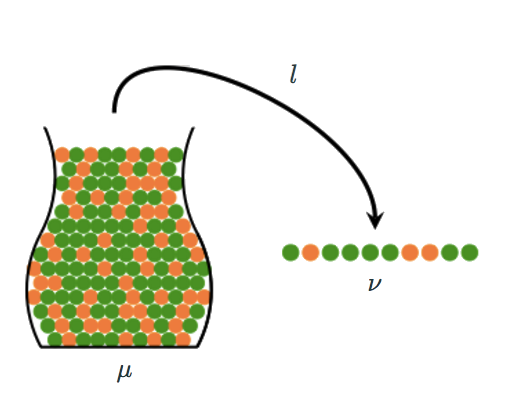
\includegraphics[width=\textwidth, keepaspectratio]{images/bin}    
      \end{figure}
    \end{center}

  \end{minipage}%
    \bigbreak
    $\nu$ -- доля оранжевых шаров в выборке размера $l$\\
    $\mu$ -- истинная доля оранжевых шаров в данных 
  
\end{frame}

\section{Какое отношение это имеет к нашим гипотезам?}

\begin{frame}
  Каждый шар это объект $x$ из пространства $X$.\\
  Неизвестная целевая функция $f$.\\
  \bigbreak
  Оранжевый шар -- гипотеза $h$ верна ($h(x) = f(x)$)\\
  Зелёный шар -- гипотеза $h$ не верна ($h(x) \neq f(x)$)\\
  \bigbreak
  По выборке $X^l$ можем оценить $\nu$ -- долю объектов, на которых верна гипотеза.
\end{frame}

\begin{frame}{Модель}
  \begin{tikzpicture}[node distance=1cm, scale=0.8, transform shape]
    \node[mynode, text width=5cm] (target) 
      {Неизвестная целевая функция\\
      \textcolor{blue}{$f: X \rightarrow Y$}};
    \node[mynode, text width=3.5cm, below=1cm of target] (training) 
      {Обучающая выборка\\
      \textcolor{blue}{${X^l = (}\textcolor{orange}{x_i}\textcolor{blue}{, y_i)_{i=1}^l}$}}
          edge[pil, <-] (target.south);
    \node[below=1cm of training] (dummy) {}; 
    \node[mycircle,text width=1.5cm, below=1cm, right=2cm of dummy] (learning) 
      {Метод обучения\\
      \textcolor{blue}{$A$}}
      edge[pil, <-, bend left=15] (training.south);  
    \node[mynode, text width=3cm, below=1cm of dummy] (hypothesis) 
      {Набор гипотез\\
      \textcolor{blue}{$\mathcal{H}$}}
      edge[pil, bend left=15] (learning.west);  
    \node[mynode, text width=3.5cm, right=1cm of learning] (final) 
      {Финальная гипотеза\\
      \textcolor{blue}{$a: h \approx f$}}
      edge[pil, <-] (learning.east);    
      
    \node[mynode, orange, right=1cm of target, text width=5cm] (probability) 
      {Вероятностное распределение\\
      \textcolor{blue}{$P$ на $X$}}
      edge[pil, bend left=35] (training.east);  
  \end{tikzpicture}
\end{frame}

\begin{frame}{$E_{in}$ и $E_{out}$}
  $E_{in}(h) = \nu$ - доля объектов в выборке $X^l$, на которых $h$ верна\\
  $E_{out}(h) = \mu$ - доля объектов во всём множестве $X$, на которых $h$ верна\\
  \bigbreak
  $$P[\vert E_{in}(h) - E_{out}(h) \vert < \varepsilon ] \leq 2 e^{-2 \varepsilon^2 l} $$\\
  \bigbreak
  Неравенство выполняется для каждой гипотезы.
\end{frame}

\begin{frame}{Важная деталь}
  \centering
  Какова вероятность, что гипотеза $a \in \mathcal{H}$, наилучшим образом приближающая $f$ по выборке, наилучшим образом приближает $f$ на всём множестве?
\end{frame}

\begin{frame}{Простая аналогия}
  \centering
  С какой вероятностью монета, подброшенная 10 раз, выпадет одной и той же стороной все 10 раз?
  \pause
  \bigbreak
  \textcolor{blue}{$0.001$}
\end{frame}

\begin{frame}{Простая аналогия}
  \centering
  С какой вероятностью одна из 1000 монет, каждая из которых подброшена 10 раз, выпадет одной и той же стороной все 10 раз?
  \pause
  \bigbreak
  \textcolor{blue}{$0.63$}
\end{frame}

\begin{frame} {К нашей задаче}
  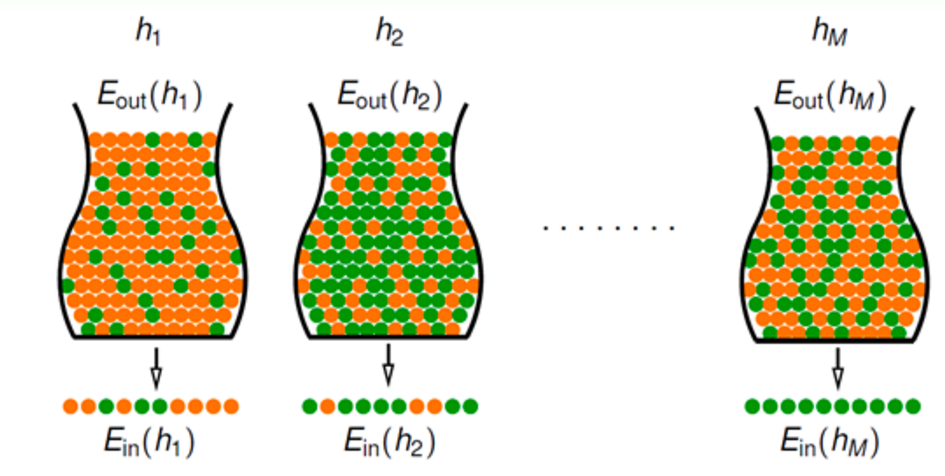
\includegraphics[width=\textwidth, keepaspectratio]{images/bins}
  
  На $h_M$ гипотезе наблюдаем переобучение.
\end{frame}

\begin{frame} {Решение}
  \begin{align*}
    P[\vert E_{in}(a) - E_{out}(a) \vert < \varepsilon ] &\leq \sum\limits_{m=1}^M P[\vert E_{in}(h) - E_{out}(h) \vert < \varepsilon ] \\
    & \leq 2\textcolor{orange}{M} e^{-2 \varepsilon^2 l} 
  \end{align*}
\end{frame}

%{\foot{loss function}
%\begin{frame}{Функция потерь}
%  Функция потерь $\mathcal{L}(a, x_i) $ -- характеризует величину ошибки алгоритма $a$ на объекте $x_i$.\\
%  \bigbreak
%  Если $\mathcal{L} (a, x_i) = 0$, то ответ $a(x_i)$ называется корректным.
%\end{frame}
%}

{\foot{loss function}
\begin{frame}{Функция потерь}
  Задача классификации:\\
  $\mathcal{L}(h, x_i) = [h(x_i) \neq y_i]$ -- индикатор ошибки\\
  \bigbreak
  Задача регрессии:\\
  $\mathcal{L}(h, x_i) = \vert h(x_i) - y_i \vert$ -- абсолютное значение ошибки\\
  $\mathcal{L}(h, x_i) = (h(x_i) - y_i)^2$ -- квадратичная ошибка\\
\end{frame}
}

{\foot{функционал средних потерь, Empirical Risk}
\begin{frame}{Функционал качества}
  Функционал качества гипотезы $h$ на выборке $X^l$:\\
  $$E_{in}(h, X^l) = \frac{1}{l} \sum\limits_{i=1}^l \mathcal{L}(h, x_i)$$\\
  Минимизация эмпирического риска:\\
  $$\arg\min\limits_{h} E_{in}(h, X^l)$$
\end{frame}
}

\begin{frame}{Полная и поточечная ошибка}  
  $$E_{in}(h, X^l) = \frac{1}{l} \sum\limits_{i=1}^l \mathcal{L}(h, x_i)$$\\
  \bigbreak
  $$E_{out} = \mathbb{E}_x \mathcal{L}(h, x) $$
\end{frame}

%\begin{frame}{Шум в наблюдениях}  
%  Что делать, если два абсолютно одинаковых объекта выборки (с точки зрения параметров) имеют разные значения $y$?
%\end{frame}
%
%\begin{frame}{Шум в наблюдениях}  
%  Будем использовать целевое распределение вместо целевой функции:\\
%  $$p(y|x)$$\\
%  Пара $(x, y)$ генерируется распределением:\\
%  $$P_x p(y|x)$$\\
%  Целевая функция выглядит так:\\
%  $f(x) = \mathbb{E}(y|x)$ + шум $y - f(x)$
%\end{frame}

\begin{frame}{Обучение в терминах вероятности}  
  В идеале хотим достичь $E_{out}(a) = 0$\\
  \bigbreak
  Пытаемся достичь $E_{in}(a) \approx E_{out}(a)$ и $E_{in}(a) = 0$
  \bigbreak
  \pause
  Два вопроса:\\
  \begin{enumerate}
    \item Можно ли судить о $E_{out}$ по $E_{in}$?
    \item Как уменьшить $E_{in}$?
  \end{enumerate}
\end{frame}

\begin{frame}{Сложность модели}  
  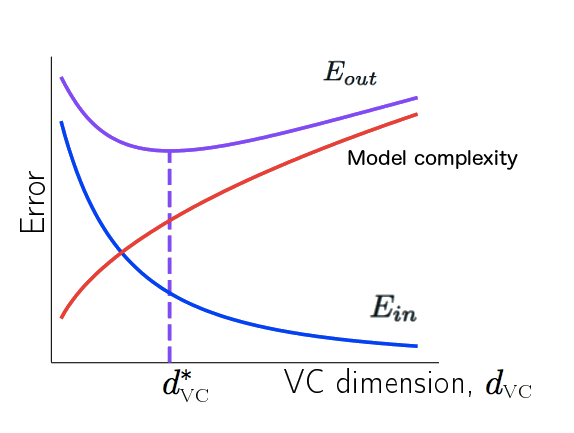
\includegraphics[ width=\textwidth, keepaspectratio]{images/vc}
\end{frame}

\section{Какое количество гипотез в нашем пространстве $\mathcal{H}$?}

\begin{frame}{Близость гипотез} 
  \centering 
  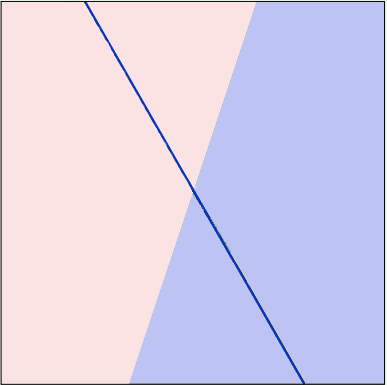
\includegraphics[ width=0.6 \textwidth, keepaspectratio]{images/hypothesis1}
\end{frame}

\begin{frame}{Близость гипотез}  
  \centering
  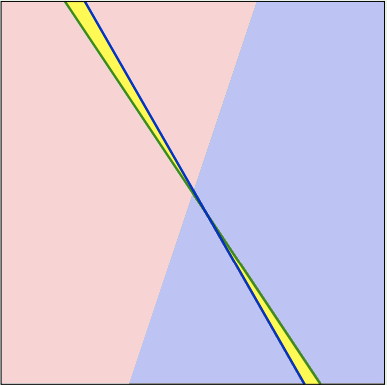
\includegraphics[ width=0.6 \textwidth, keepaspectratio]{images/hypothesis}
\end{frame}

\begin{frame}{Близость гипотез}  
  $\bigtriangleup E_{out} = $ площадь жёлтой области\\
  \bigbreak
  $\bigtriangleup E_{in} = $ изменение меток объектов жёлтой области в выборке\\
  \bigbreak
  $\vert E_{in}(h_1) - E_{out}(h1) \vert \approx \vert E_{in}(h_2) - E_{out}(h2) \vert$  
\end{frame}

\begin{frame}{Вопрос}  
  \begin{minipage}[t]{0.5\linewidth}
    \begin{flushleft}
    Обучающая выборка $x_1, \dots, x_l$ и набор бинарных значений меток $y_1,\dots,y_l$.\\
    \end{flushleft}
  \end{minipage}%
  \begin{minipage}{0.5\linewidth}
      \centering
        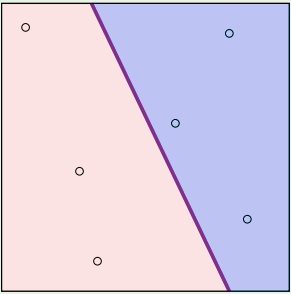
\includegraphics[width=0.8 \textwidth, keepaspectratio]{images/dich}    
  \end{minipage}%  
  \centering  
  \bigbreak
  Сколько вариантов $y_1,\dots, y_l$? 
\end{frame}

{\foot{коэффициент разнообразия}
\begin{frame}{Дихотомии}  
  $$P(\vert E_{in}(a) - E_{out}(a) \vert > \varepsilon) \leq 2 M e^{-2\varepsilon^2l}$$  \\
  Наш набор гипотез $\mathcal{H}$ может породить $\vert \mathcal{H}(x_1,\dots, x_l) \vert$ дихотомий.\\
  $$\vert \mathcal{H}(x_1,\dots, x_l) \vert \leq 2^l$$\\
  При этом сам набор гипотез может быть бесконечным.
\end{frame}
}

\begin{frame}{Функция роста $m_{\mathcal{H}(l)}$}  
  \centering
  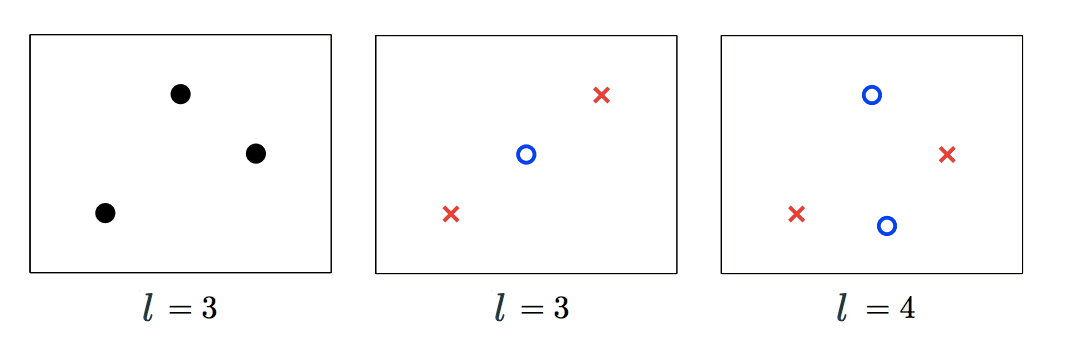
\includegraphics[width=\textwidth, keepaspectratio]{images/growth}
  $$m_{\mathcal{H}(l)} = \max\limits_{x_1,\dots,x_l} \vert \mathcal{H}(x_1,\dots, x_l) \vert$$\\
  $$m_{\mathcal{H}(l)} \leq 2^l$$\\
\end{frame}

\begin{frame} {Функция роста $m_{\mathcal{H}(l)}$}
  Гипотезы:\\  
  \begin{enumerate}
    \item Луч на множестве точек: $m_{\mathcal{H}}(l) = l+1 $
    \item Интервал на множестве точек: $m_{\mathcal{H}}(l) = C_{l+1}^2 + 1$
    \item Выпуклое множество на множестве точек: $m_{\mathcal{H}}(l) = 2^l$ 
  \end{enumerate}
\end{frame}

{\foot{точка поломки, break point}
\begin{frame}{Точка разрыва}  
  Если для некоторого $k$ выполняется $m_{\mathcal{H}}(k) < 2^k$, то $k$ называется точкой разрыва.
\end{frame}
}

\begin{frame}{Точка разрыва}  
  \centering
  Наличие точки разрыва означает наличие полиномиального ограничения на функцию роста $m_{\mathcal{H}}(l)$
\end{frame}

\begin{frame}{Пример}  
  \centering
  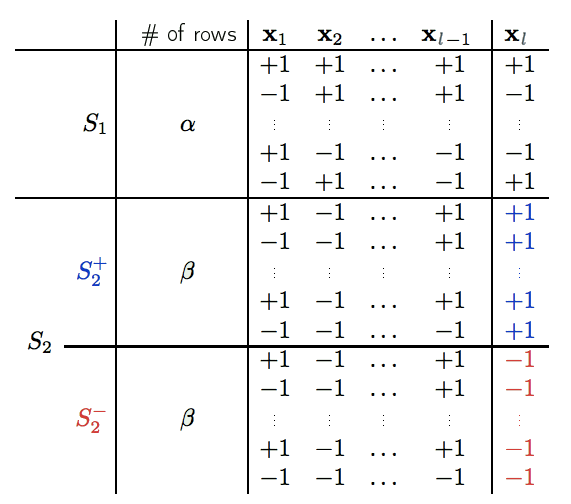
\includegraphics[width=\textwidth, height=0.8 \textheight, keepaspectratio]{images/breakpoint}\\
  Разделим на 2 ситуации относительно $x_l$: \\либо есть только один вариант (+1 или -1), либо оба (+1 и -1)
\end{frame}

\begin{frame}{Число дихотомий}  
  $B(l, k)$ -- максимальное число дихотомий для выборки размера $l$ при наличии точки разрыва $k$.\\
  \bigbreak
  \begin{itemize}
    \item $B(l, k) = \alpha  + 2\beta$
    \item $\alpha + \beta \leq B(l-1, k)$, т.к. $\alpha + \beta$ -- число дихотомий для $l-1$\\
    \item $\beta \leq B(l-1, k-1)$ 
  \end{itemize}
  $\implies B(l, k) \leq B(l-1, k) + B(l-1, k-1)$
\end{frame}

\begin{frame}{Число дихотомий}  
  $$B(l, k) \leq \sum\limits_{i=0}^{k-1} C_l^i$$\\
  Доказывается по индукции.\\
  Индукционный шаг:
  $$\sum\limits_{i=0}^{k-1} C_l^i = \sum\limits_{i=0}^{k-1} C_{l-1}^i + \sum\limits_{i=0}^{k-2} C_l^i$$
\end{frame}

\begin{frame}{Полиномиальное ограничение}  
  $$m_{\mathcal{H}(l)} \leq \sum\limits_{i=0}^{k-1} C_l^i$$\\
  Доказывается по индукции.\\
  Индукционный шаг:
  $$\sum\limits_{i=0}^{k-1} C_l^i = \sum\limits_{i=0}^{k-1} C_{l-1}^i + \sum\limits_{i=0}^{k-2} C_l^i$$
\end{frame}

\begin{frame}{Неравенство Вапника-Червоненкиса}  
  $$P(E_{in}(a) - E_{out}(a) > \varepsilon) \leq 4 m_{\mathcal{H}}(2l) e^{-\frac{1}{8}\varepsilon^2l}$$\\
  \bigbreak
  Размерность $d_{VC} = $ наибольшее $l$, для которого $m_{\mathcal{H}}(l) = 2^l$. $d_{VC} = k-1$.
  
\end{frame}

\begin{frame}{Регуляризация}  

\end{frame}

\begin{frame}{Кроссвалидация}  

\end{frame}

\begin{frame}{Генерация модельных данных}  

\end{frame}

\begin{frame}[standout]
  Вопросы?
\end{frame}

\appendix

\begin{frame}\frametitle{На следующей лекции}
	\begin{itemize}
    	\item[--] Функционалы качества
    	\item[--] Неравенство Хефдинга
    	\item[--] Близость гипотез
    	\item[--] Неравенство Вапника-Червоненкиса
    	\item[--] Генерация модельных данных    	    	
	\end{itemize}
\end{frame}
\end{document}

\end{document}